\documentclass[a4paper]{article}

\usepackage{INTERSPEECH2016}

\usepackage{graphicx}
\usepackage{amssymb,amsmath,bm}
\usepackage{textcomp}
\usepackage{verbatim}
\def\vec#1{\ensuremath{\bm{{#1}}}}
\def\mat#1{\vec{#1}}


\sloppy % better line breaks
\ninept

\title{Segmentation of birdsong}

%%%%%%%%%%%%%%%%%%%%%%%%%%%%%%%%%%%%%%%%%%%%%%%%%%%%%%%%%%%%%%%%%%%%%%%%%%
%% If multiple authors, uncomment and edit the lines shown below.       %%
%% Note that each line must be emphasized {\em } by itself.             %%
%% (by Stephen Martucci, author of spconf.sty).                         %%
%%%%%%%%%%%%%%%%%%%%%%%%%%%%%%%%%%%%%%%%%%%%%%%%%%%%%%%%%%%%%%%%%%%%%%%%%%
%\makeatletter
%\def\name#1{\gdef\@name{#1\\}}
%\makeatother
%\name{{\em Firstname1 Lastname1, Firstname2 Lastname2, Firstname3 Lastname3,}\\
%      {\em Firstname4 Lastname4, Firstname5 Lastname5, Firstname6 Lastname6,
%      Firstname7 Lastname7}}
%%%%%%%%%%%%%%% End of required multiple authors changes %%%%%%%%%%%%%%%%%

\makeatletter
\def\name#1{\gdef\@name{#1\\}}
\makeatother \name{{\em Author Name$^1$, Co-author Name$^2$}}

\address{$^1$Author Affiliation \\
  $^2$Co-author Affiliation \\
  {\small \tt author@university.edu, coauthor@company.com}
}

%\twoauthors{Karen Sp\"{a}rck Jones.}{Department of Speech and Hearing \\
%  Brittania University, Ambridge, Voiceland \\
%  {\small \tt Karen@sh.brittania.edu} }
%  {Rose Tyler}{Department of Linguistics \\
%  University of Speechcity, Speechland \\
%  {\small \tt RTyler@ling.speech.edu} }

%
\begin{document}

  \maketitle
  %
  \begin{abstract}
  \end{abstract}
  \noindent{\bf Index Terms}: speech recognition, human-computer interaction, computational paralinguistics



  \section{Introduction}

\section{Entropy-based segmentation of birdsong}
This section describes how to calculate entropy from spectrogram and phase spectrum, also how to use entropy to identify bird vocalizations. The entropy of spectrograms of bird song recordings can be effectively used for distinguishing between background and bird vocalizations \cite{6625329}. Spectrogram of single bird song is generally sparse i.e. high power components acquire only a small portion of time-frequency bins and the background noise of spectrogram is relatively white. Hence  the entropy of sliding time frequency block over spectrogram is low when block contains a signal and is high when only background is present in that block. It is known that phase spectrum has more information than magnitude spectrum. So, phase spectrum can also be used to calculate entropy. Group delay functions from all pole models are used to calculate the phase spectrum. 

\subsection{Entropy Calculation}
Entropy is calculated for each time-frequency block on power spectrum. This time-frequency block of time length \textbf{\textit{w}} and having F frequency bins ranging from \textbf{\textit{f1}} to  \textbf{\textit{fn}} is moved horizontally from beginning to the end of power spectrum. The frequency range is different for each target species. \textbf{\textit{p(n,f)}} is power spectrum at time \textbf{\textit{n}} and frequency  \textbf{\textit{f}}. The entropy is calculated using following equation:

\hspace{1cm}

  $h_{k}=\sum_{n=kT+1}^{kT+w}\sum_{f=f1}^{fn}z(n,f) \ln z(n,f)$

 \hspace{1cm}
 
Here \textbf{\textit{T}} is time-frequency block shift and \textbf{\textit{z(n,f)}} is normalized power spectrum.


\hspace{1cm}

$z(n,f)=\frac {p(n,f)}
{\sum_{n=kT+1}^{kT+w}\sum_{f=f1}^{fn} p(n,f)}$

\hspace{1cm}


The entropy calculated from block is less susceptible to the bursts of background noise in comparison to the entropy calculated at each time instance. 


\subsection{Whitening Spectrogram before Entropy Calculation}

To identify the bird vocalizations using entropy, there should be a clear distinction between the entropy of background and call period. However this is not always the case in raw sound recordings. Depending on the interference level, entropy at a quiet period can even be higher than the entropy at a call period or bird call activity [1]. To overcome this problem, whole spectrogram or power spectrum is whitened using PCA  before calculating entropy. The entropy calculated from whitened spectrogram is almost constant for background but dips enough to mark the presence of bird vocalizations. Even low energy bird vocalizations can be detected accurately using this method. The missed detection rate is decreased if whitened spectrogram is used for entropy calculation. 

To whiten the spectrogram (\textit{PS}), the covariance matrix of mean subtracted spectrogram is calculated. The Eigen values matrix (\textit{S}) and Eigen vectors matrix (\textit{U}) of this covariance matrix are calculated. The spectrogram matrix is whitened using the following equation:

\hspace{1cm}

$WhitePS=diag(\frac{1}{\sqrt{diag(S)+\epsilon}})*\textit{U'}*\textit{PS}$


\hspace{1cm}


Figure 1 depicts the difference between entropy calculated from normal spectrogram and whitened spectrogram:
\begin{figure}[!ht]
	\centering
	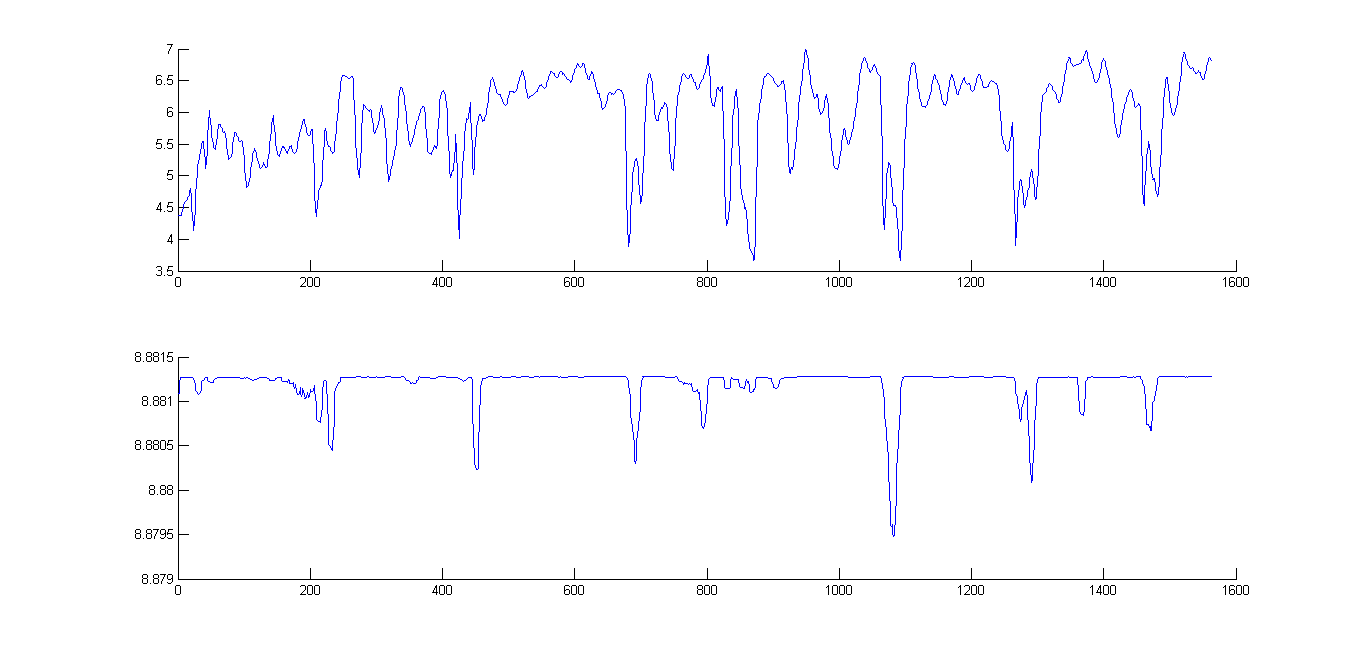
\includegraphics[width=8cm, height=6cm]{entropy}
	\caption{ Entropy calculated from normal spectrogram and whitened spectrogram}   
\end{figure}

It becomes evident that identifying bird vocalizations using entropy calculated from whitened spectrogram is easier.  



\subsection{Entropy Calculation from phase spectrum}



\subsection{Detecting change points using thresholding}

To detect the change points, thresholding is used. The local minimums and local maximums are calculated on the  entropy. The difference between consecutive local minimums and local maximums is calculated. If this difference is greater than pre-defined threshold, then corresponding local maximum is considered as the start of a bird vocalization or a change point. Then the difference between corresponding local minima and next local maxima is calculated. If this difference is greater than the threshold, local maxima is considered as the end of bird vocalization or another change point. Hence two contiguous change points correspond to the start and end of a bird vocalization. These change points can be tracked back to get the start and end time of the vocalization in sound recording. Figure 2 shows the local maximums and local minimums on an entropy plot along with change points calculated from thresholding.

\begin{figure}[!ht]
	\centering
	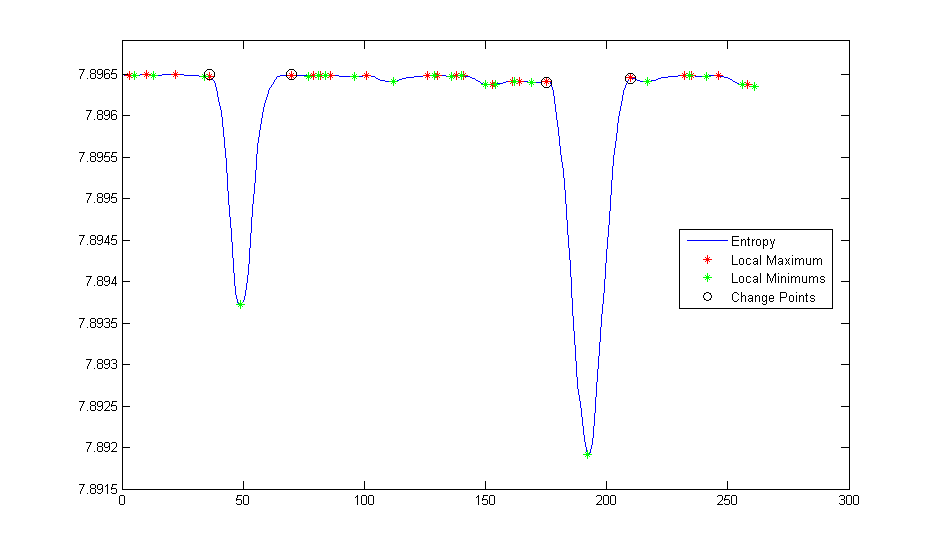
\includegraphics[width=9cm, height=4cm]{thresholding}
	\caption{ Change points generated by thresholding and Extrema calculated on entropy}   
\end{figure} 

   




\section{Experimentation and Performance Analysis}

For experimentation, the labeled recordings of Cassin’s Vireo (\textit{Vireo cassinii}) and single species MLSP Bird Classification Challaenge 2013 datasets are used \cite{data}. 

In Cassin's Vireo dataset, the total duration of recordings is about 45 minutes. Out of 45 minutes, about 5 minutes of recordings correspond to the phrases of Cassin's Vireo. To calculate spectrogram, frame length of 20 ms and increment of  
5 ms is used. The time-frequency window of 138.8 ms is used along with increment of 15 ms to calculate entropy. The frequency range of the block is from 1.5 kHz to 7 kHz.  

The method is analyzed using manual annotations of bird vocalizations. For performance analysis, three metrics i.e. true positive rate, missed detection rate and false alarm rate are used. These metrics are calculated using following equations:\newline



$\text{True Positive rate (\%)}=\frac{\text{Frames correctly classified as calls}} {\text{Total frames contating call activity}} \times 100$\newline


$\text{Missed Detection (\%)}=\frac{\text{Frames  misclassified as background}} {\text{Total call activity frames}} \times 100$\newline

$\text{False Alarms (\%)}=\frac{\text{Background  frames classified as calls}} {\text{Total background frames}} \times 100$ \newline



 ROC curves are used for analyzing the method. Figure 3 depicts ROC curves comparing performance of methods based on entropy calculated from whitened spectrogram and entropy calculated from whitened group delay phase spectrum. It is clear from ROC plot in Figure 3 that whitened Group delay phase spectrum method is outperforming whitened power spectrum method.


\begin{figure}[!ht]
	\centering
	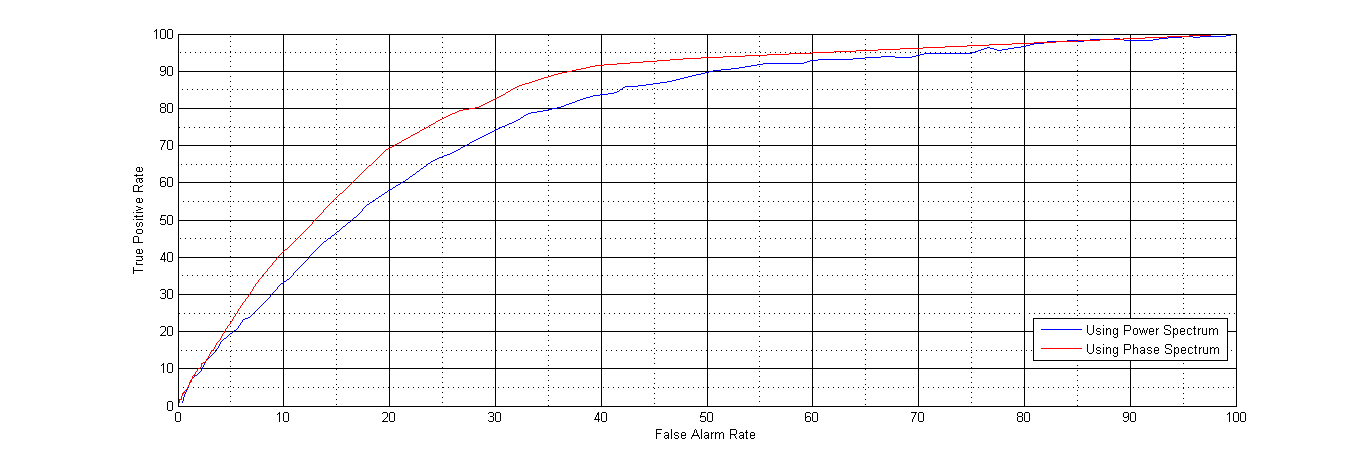
\includegraphics[width=9cm, height=5cm]{Power_vs_phase_white}
	\caption{ROC curves comparing white phase spectrum and white power spectrum methods}   
\end{figure} 



The effect of whitening the phase spectrum before entropy calculation is evident from the ROC curves depicted in Figure 4 and Figure 5. The analysis of ROC in Figure 4 establishes that whitening the phase spectrum gives better performance than using phase spectrum which is not whitened. 

\begin{figure}[!ht]
	\centering
	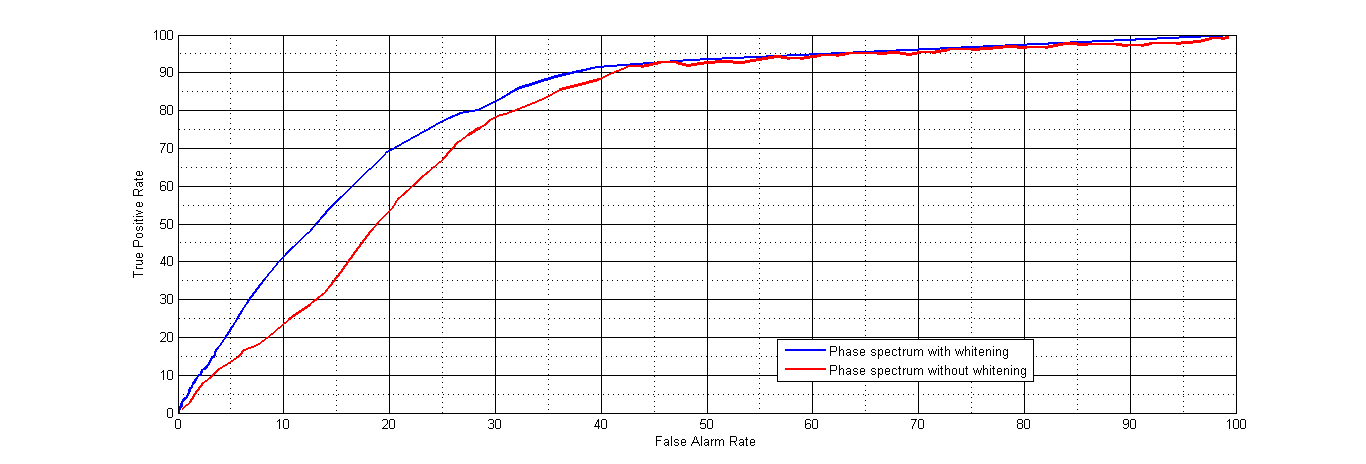
\includegraphics[width=9cm, height=5cm]{phase_non_white_vs_phase_white}
	\caption{ROC curves comparing performance of methods based whitened phase spectrum and non white phase spectrum}   
\end{figure} 
 
 Figure 5 shows comparison of ROC plots between methods based on white and non white power spectrum. 
 
 \begin{figure}[!ht]
 	\centering
 	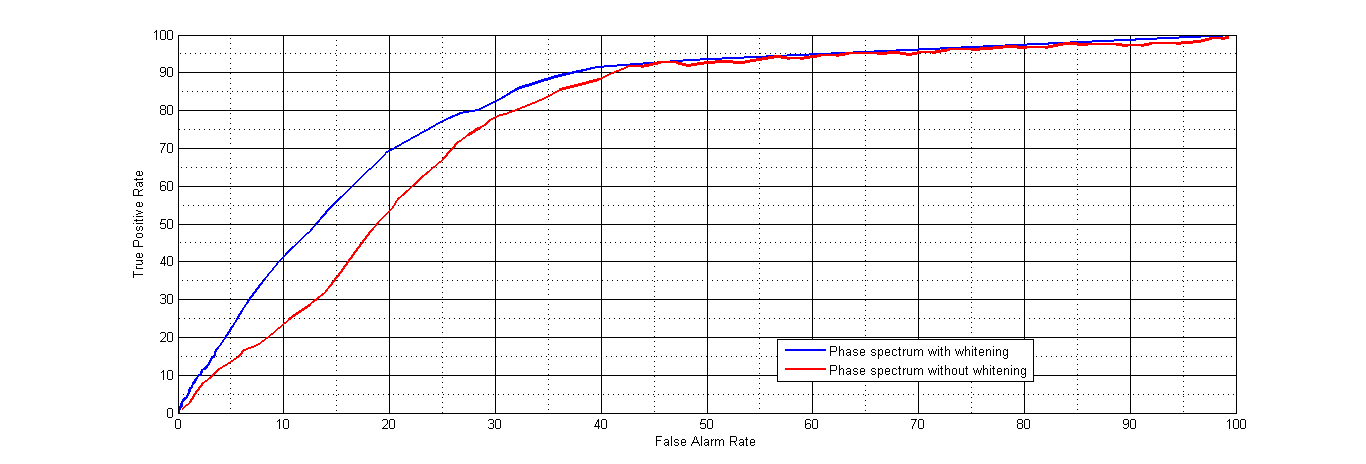
\includegraphics[width=9cm, height=5cm]{phase_non_white_vs_phase_white}
 	\caption{ROC curves comparing performance of methods based whitened power spectrum and non white power spectrum}   
 \end{figure} 
 
 
 
 
The method is also evaluated on an another dataset i.e. single species MLSP Bird Classification Challaenge 2013. The recordings have low signal to noise ratio.  Figure 6 shows ROC curves comparing performance of methods based on entropy calculated from whitened spectrogram and entropy calculated from whitened group delay phase spectrum on single species MLSP data.

 
\begin{figure}[!ht]
	\centering
	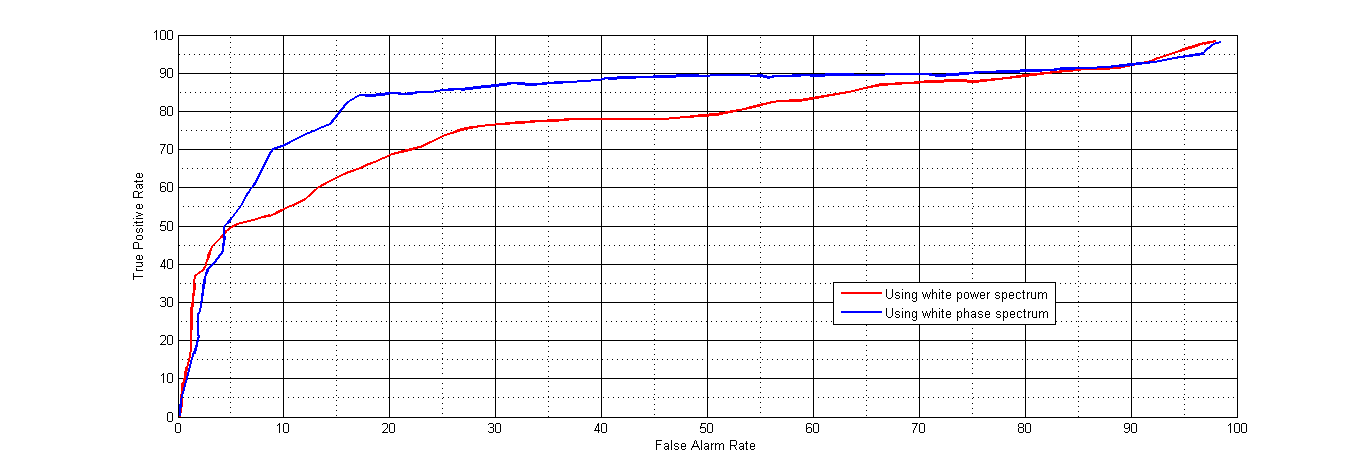
\includegraphics[width=9cm, height=4cm]{ROC_data_2_gd_vs_spectogram_white}
	\caption{ROC curves comparing performance of methods based on white phase spectrum and white power spectrum on MLSP 2013 single species dataset }   
\end{figure} 

 



%%  write formullae for calculating correct, missed detection and false alarms
\begin{comment}
Table 1 shows results generated by applying entropy based segmentation with thresholding on different sound recordings. 

  



\begin{table}[]
	\centering
	\caption{Table showing Correct (\%) Missed Detection(\%) and False alarm (\%) for particular thresholds and moving average windows } 
	\label{Table 1}

	\begin{tabular}{|c|c|c|c|c|c|}
		\hline
		\textbf{File} & \textbf{Span} & \textbf{Threshold} & \textbf{Correct (\%)} & \textbf{False Alarm (\%)} & \textbf{Missed Detection (\%)} \\ \hline
		1.wav         & 9             & 1.2                & 77.7                  & 15.6                      & 60.5                           \\
	\hline	2.wav         & 3             & 1.45               & 73                    & 45                        & 25                             \\
		\hline	3.wav         & 3             & 1.5                & 71                    & 22                        & 54                             \\
		\hline	4.wav         & 9             & 1.15               & 75.1              & 21                  & 51.5                       \\
		\hline	5.wav         & 7             & 1.5                & 76.5                  & 18.5                      & 45                             \\
	\hline		6.wav         & 9             & 1.25               & 82.1              & 15.07                  & 32.2                       \\
		\hline	7.wav         & 7             & 1.25               & 79.6              & 17.8                  & 46.7                       \\
		\hline	8.wav         & 9             & 1.15               & 78.8              & 19.3                  & 35.1                      \\
		\hline	9.wav         & 5             & 1.5                & 86.06              & 13.6                  & 17.9                       \\
	\hline		10.wav        & 9             & 1.6                & 79.6              & 18.3                  & 28.31                       \\
		\hline	11.wav        & 3             & 1.45               & 91.1                  & 32.7                      & 7.53                           \\
		\hline	12.wav        & 7             & 1.4                & 85.1              & 11.3                   & 38.1      \\ \hline               	
	 
	\end{tabular}

\end{table}

\end{comment}
 
 
\section{Conclusion}
We propose an entropy based bird vocalization segmentation method where entropy is calculated from Group Delay phase spectrum. It is also established that whitening the power or phase spectrum before entropy calculation improves the performance of entropy based segmentation. From experimentation,it is clear that the proposed group delay based method outperforms the power spectrum based method.  



  \newpage
  \eightpt
  \bibliographystyle{IEEEtran}

  \bibliography{mybib}

%  \begin{thebibliography}{9}
%    \bibitem[1]{Davis80-COP}
%      S.\ B.\ Davis and P.\ Mermelstein,
%      ``Comparison of parametric representation for monosyllabic word recognition in continuously spoken sentences,''
%      \textit{IEEE Transactions on Acoustics, Speech and Signal Processing}, vol.~28, no.~4, pp.~357--366, 1980.
%    \bibitem[2]{Rabiner89-ATO}
%      L.\ R.\ Rabiner,
%      ``A tutorial on hidden Markov models and selected applications in speech recognition,''
%      \textit{Proceedings of the IEEE}, vol.~77, no.~2, pp.~257-286, 1989.
%    \bibitem[3]{Hastie09-TEO}
%      T.\ Hastie, R.\ Tibshirani, and J.\ Friedman,
%      \textit{The Elements of Statistical Learning -- Data Mining, Inference, and Prediction}.
%      New York: Springer, 2009.
%    \bibitem[4]{YourName16-XXX}
%      F.\ Lastname1, F.\ Lastname2, and F.\ Lastname3,
%      ``Title of your INTERSPEECH 2016 publication,''
%      in \textit{Interspeech 2016 -- 16\textsuperscript{th} Annual Conference of the International Speech Communication Association, September 8–12, San Francisco, California, USA, Proceedings, Proceedings}, 2016, pp.~100--104.
%  \end{thebibliography}

\end{document}
